\documentclass[tikz,border=5pt]{standalone}
\usepackage{pgfplots}
\pgfplotsset{/pgf/number format/use comma,compat=1.16}
\usepackage[T1]{fontenc}
\usepackage[utf8]{inputenc}
\usepackage{stanli} % TikZ Library for Structural Analysis by Jurgen Hackl
\usetikzlibrary{calc,intersections,patterns}

\begin{document}
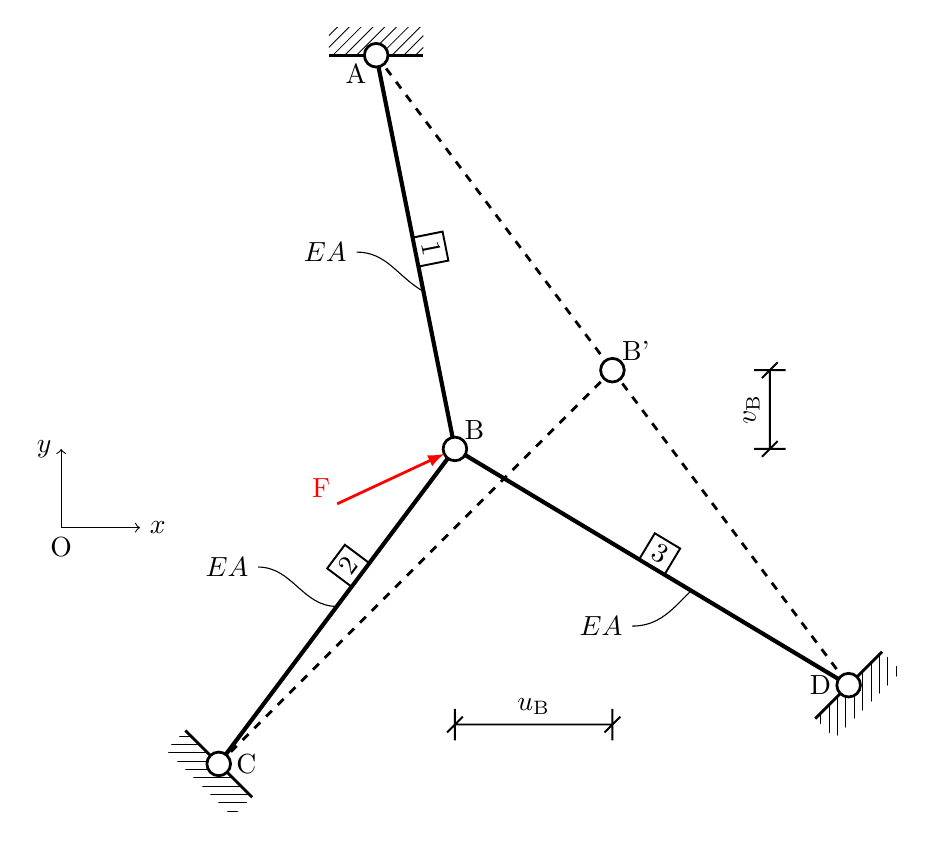
\begin{tikzpicture}[scale=1]
  %\draw [help lines] (0,0) grid [step=1] (8,9); %useful for construction
  % origin of the coordinates system
  \draw (-2,3) node[below] {O};
  %coordinates system
  \draw[<->] (-1,3) node[right] {$x$}-|(-2,4) node[left]{$y$};
  %point
  \point{A}{2}{9};
  \point{B}{3}{4};
  \point{B'}{5}{5};
  \point{C}{0}{0};
  \point{D}{8}{1};
  %beams
  \beam{2}{A}{B}[0][0];
  \beam{2}{B}{C}[0][0];
  \beam{2}{B}{D}[0][0];
  \beam{3}{A}{B'};
  \beam{3}{B'}{C};
  \beam{3}{B'}{D};
  \notation{4}{A}{B}[1];
  \notation{4}{C}{B}[2][0.6];
  \notation{4}{D}{B}[3];
  %supports
  \support{3}{A}[180];
  \support{3}{C}[-45];
  \support{3}{D}[45];
  %hinges
  \hinge{1}{A}
  \hinge{1}{B}
  \hinge{1}{C}
  \hinge{1}{D}
  \hinge{1}{B'}
  %load force
  \begin{scope}[color=red]
    \load{1}{B}[205][1.5];
    \notation{1}{1.3,3.5}{F}[centered];
  \end{scope}
  %displacements
  \dimensioning{1}{B}{B'}{0.5}[$u_\mathrm{B}$];
  \dimensioning{2}{B}{B'}{7}[$v_\mathrm{B}$];
  %labels
  \notation{1}{A}{A}[below left];
  \notation{1}{B}{B}[above right];
  \notation{1}{B'}{B'}[above right];
  \notation{1}{C}{C}[right=1mm];
  \notation{1}{D}{D}[left=1mm];
  \draw (0.5,2.5) node[left]{$EA$} to [out=0,in=180] (1.5,2);
  \draw (1.75,6.5) node[left]{$EA$} to [out=0,in=150] (2.6,6);
  \draw (5.25,1.75) node[left]{$EA$} to [out=0,in=225] (6,2.2);
  % To-paths are really useful for drawing curved lines. The above
  % to path is equal to:
  %
  % \draw[-latex,thick] (3.2,0.5) node[right]{$\mathsf{S_{1,2}}$}
  %      ..controls +(180:.2cm) and +(up:0.25cm) .. (3,0);
  % Internally the to path is translated to a similar bezier curve,
  % but the to path syntax hides the complexity from the user.
\end{tikzpicture}
\end{document}